\documentclass[12pt,a4paper]{report}

% Encoding & Layout
\usepackage[utf8]{inputenc}
\usepackage{geometry}
\geometry{a4paper, margin=1in}

% Graphics & Links
\usepackage{graphicx}
\usepackage{hyperref}

% Color Palette (Elegant Purple + Gold)
\usepackage{xcolor}
\definecolor{primary}{RGB}{88, 24, 69}      % Deep Purple
\definecolor{secondary}{RGB}{199, 161, 122} % Soft Gold
\definecolor{accent}{RGB}{245, 240, 250}    % Light background

% Header/Footer
\usepackage{fancyhdr}

% Section Styling
\usepackage{titlesec}

% Tables & Listings
\usepackage{booktabs}
\usepackage{tabularx}
\usepackage{listings}

% Figures & Mathematics
\usepackage{caption}
\usepackage{subcaption}
\usepackage{amsmath,amssymb,amsthm}
\usepackage{float}

% Lists & References
\usepackage{enumitem}
\usepackage{cleveref}

% TikZ for borders
\usepackage{tikz}
\usetikzlibrary{positioning}

% DOUBLE BORDER DESIGN
\usepackage{eso-pic}
\AddToShipoutPictureBG{
\begin{tikzpicture}[remember picture,overlay]

    % Outer Border
    \draw[line width=2pt, color=primary!70] 
        ([shift={(0.8cm,-0.8cm)}]current page.north west) 
        rectangle 
        ([shift={(-0.8cm,0.8cm)}]current page.south east);

    % Inner Border
    \draw[line width=0.8pt, color=secondary!80] 
        ([shift={(1.2cm,-1.2cm)}]current page.north west) 
        rectangle 
        ([shift={(-1.2cm,1.2cm)}]current page.south east);

\end{tikzpicture}
}

% Hyperref Setup
\hypersetup{
    colorlinks=true,
    linkcolor=primary,
    urlcolor=secondary,
    pdftitle={Project Vanish Lite Report}
}

% Header/Footer Styling
\pagestyle{fancy}
\fancyhf{}
\lhead{\textcolor{primary}{Project Vanish Lite}}
\rhead{\textcolor{secondary}{PDP Report}}
\cfoot{\thepage}

% CENTERED CHAPTER STYLE
\titleformat{\chapter}[display]
  {\normalfont\huge\bfseries\centering\color{primary}}
  {}
  {0pt}
  {\vspace{2cm}
   \textcolor{secondary}{\rule{0.5\textwidth}{1pt}}\\[1ex]
   \Huge \bfseries}
  [\vspace{1ex}\textcolor{secondary}{\rule{0.5\textwidth}{1pt}}]

% Section Styling
\titleformat{\section}
  {\normalfont\Large\bfseries\color{primary}}
  {\thesection}{1em}{}

\titleformat{\subsection}
  {\normalfont\large\bfseries\color{secondary!90!black}}
  {\thesubsection}{1em}{}

% Spacing
\titlespacing*{\chapter}{0pt}{0pt}{30pt}
\titlespacing*{\section}{0pt}{12pt}{6pt}

% Code Styling
\lstset{
    basicstyle=\ttfamily\small,
    backgroundcolor=\color{accent},
    frame=single,
    rulecolor=\color{primary!40},
    breaklines=true
}

\begin{document}

% ================= TITLE PAGE =================
\begin{titlepage}
    \centering
    
\includegraphics[width=0.34\textwidth]{iiitdmk_logo.jpeg}
    
    \vspace*{2cm}
    {\Huge \bfseries \textcolor{primary}{Project Vanish Lite}\par}
    \vspace{0.5cm}
    {\Large \textcolor{secondary}{A Disposable Linux Workspace System}\par}
    \vspace{2cm}
    
    \textcolor{secondary}{\rule{\textwidth}{1.5pt}}
    \vspace{0.5cm}
    
    {\Large \textbf{Product Development Project Report}}
    \vspace{0.5cm}

    \textcolor{secondary}{\rule{\textwidth}{1.5pt}}
    
    \vspace{2cm}
    
    \begin{flushleft}
    \textbf{Submitted to:}\\
    Assistant Professor Alapan Kuila
    
    Dept of Computer Science and Engineering
    
    IIITDM Kurnool
    \end{flushleft}
    \vspace{1cm}
    \begin{flushleft}
    \textbf{Submitted by:}\\
    123CS0004 N. Pranav
    
    123CS0052 M. Vighnesh Prasad
    
    123CS0058 G. V. Sai Srivardhan
    
    123AD0023 V. Siva Sai
    \end{flushleft}
    
    \vfill
    {\large \par}
\end{titlepage}

% ================= FRONT MATTER =================
\pagenumbering{roman}
\tableofcontents
\newpage

\listoffigures
\listoftables
\newpage

% ================= MAIN CONTENT =================
\pagenumbering{arabic}

\chapter{Introduction}

\section{Abstract}
In the era of heightened digital surveillance and security breaches, ensuring a safe computing environment presents a significant challenge. Threat actors often compromise systems by injecting malicious persistence mechanisms or extracting sensitive local data. Project Vanish Lite is a robust, dynamic, and disposable Linux user workspace system designed to mitigate these threats. It provisions temporary system users, applies policy-based restrictions depending on the specific threat model (e.g., Secure, Privacy, Exam, Online), and guarantees strict teardown mechanisms that enforce zero local persistence. This project demonstrates a secure stateless computing model that effectively decouples persistent user state from the host hardware . Engineered with a C++ core engine and a scalable Python backend, Vanish Lite achieves stringent isolation through dynamic configurations and native OS features.

\section{Introduction}
Modern computing relies heavily on persistent, mutable states. While this benefits long-term user experiences, it introduces inherent vulnerabilities: a compromised device remains compromised until thoroughly remitted. Digital forensics, exam monitoring, and privacy-conscious browsing all demand environments that return to a strictly defined clean state upon session termination.

While cryptographic file systems try to conceal data, they do not inherently provide amnesia or stateless session guarantees. Virtualization tools like Docker or VMware offer sandboxing but bring significant orchestration overhead and heavy resource utilization. 

Project Vanish Lite fundamentally diverges from typical sandboxing techniques. Instead of full virtualization or containerization, it interfaces at the host OS level by managing native Linux users dynamically. By injecting specific personal data only when authorized and forcefully annihilating the entire environment at shutdown, it achieves a secure, transparent, and ephemeral architecture.

\subsection{Key Contributions}
The core contributions of this work include:
\begin{itemize}
    \item \textbf{Dynamic Lifecycle Management:} An OS-level engine orchestrating the complete lifecycle of user creation, daemon execution, and session annihilation.
    \item \textbf{Mode-Based Policy Engine:} Robust session controls mapped to predefined modes: \texttt{dev}, \texttt{secure}, \texttt{privacy}, \texttt{exam}, and \texttt{online}.
    \item \textbf{Strict Teardown Guarantee:} Resilient session cleanup sequences employing recursive kill processes hooks and enforced un-mounting mechanisms to ensure zero local persistence.
    \item \textbf{Administrative Web Interface:} An intuitive admin panel facilitating snapshot management, compliance reporting, and real-time session overview.
\end{itemize}

\chapter{Problem Statement and Scope}

\section{Problem Statement}
Existing computing models manage state persistently across user sessions, creating a multitude of issues in high-security, educational, or highly private situations:
\begin{table}[h]
    \centering
    \begin{tabularx}{\textwidth}{lX}
    \toprule
    \textbf{Limitation} & \textbf{Vanish Lite Resolution} \\
    \midrule
    State Persistence & Implements strict, resilient teardown guarantees enforcing zero local persistence through \texttt{userdel} and process termination hooks. \\
    Resource Heavy Isolation & Operates inherently on the host OS by using Linux user paradigms and local group management instead of running heavy virtual machines. \\
    Static Security Modeling & Provides dynamic mode-based policies (\texttt{dev}, \texttt{secure}, \texttt{privacy}, \texttt{exam}, \texttt{online}) configurable down to DNS resolution and USB access constraints. \\
    Complex Auditing & Implements automated per-session snapshots and compliance reports, seamlessly integrated with a management web interface. \\
    \bottomrule
    \end{tabularx}
    \caption{Limitations of traditional computing paradigms compared to Vanish Lite.}
    \label{tab:limitations}
\end{table}

The primary technological hurdle lies in engineering an extensible session enforcement mechanism that can transparently intercept operations and apply strict quotas or network allowances without requiring deep kernel module dependencies.

\section{Objectives}
The core objectives of the Project Vanish Lite platform are to:
\begin{enumerate}
    \item Design an engine that correctly performs dynamic, error-free provisioning and deprovisioning of temporary Linux user accounts.
    \item Implement tailored modes restricting CPU, memory, Network access, and specific executables using local firewall (\texttt{iptables}) commands and \texttt{cgroups}-like constraints.
    \item Create a failsafe cleanup daemon guaranteeing the absolute removal of all temporary processes and persona configurations, preventing orphan environments.
    \item Develop an intuitive Admin Dashboard providing total visibility, telemetry generation, and snapshot reviews.
\end{enumerate}

\section{Scope}
The scope of the project encompasses the development, deployment, and testing of the Linux session management engine and the web-based administrative dashboard. It natively encompasses the following components:
\begin{itemize}
    \item \textbf{C++ Enforcement Engine:} Handles system calls, handles \texttt{sigaction} loops, and invokes network rule modifiers securely.
    \item \textbf{Mode Policies:} \texttt{secure} (restricting peripheral input), \texttt{exam} (whitelisting network rules, mounting persistence drives), \texttt{privacy} (RAM-mounted home directories), and \texttt{online} (configurable dynamic networking paths).
    \item \textbf{Server API:} A Python-backend orchestrating the user interface, session history reporting, and configurations.
\end{itemize}
The current iteration targets modern Linux distributions, assuming root execution privileges for the central daemon.

\chapter{System Architecture}

\section{Overview}
Project Vanish Lite is partitioned into two primary functional halves: the low-level Local Execution System handling daemon creation and restrictions, and the higher-level Web Admin Panel orchestrating monitoring and visualization. The system operates strictly locally, eliminating the need for complex cloud orchestration components and decreasing latency natively.

\begin{figure}[htp]
    \centering
    % Placeholder for the architecture diagram which we will generate as a flowchart
    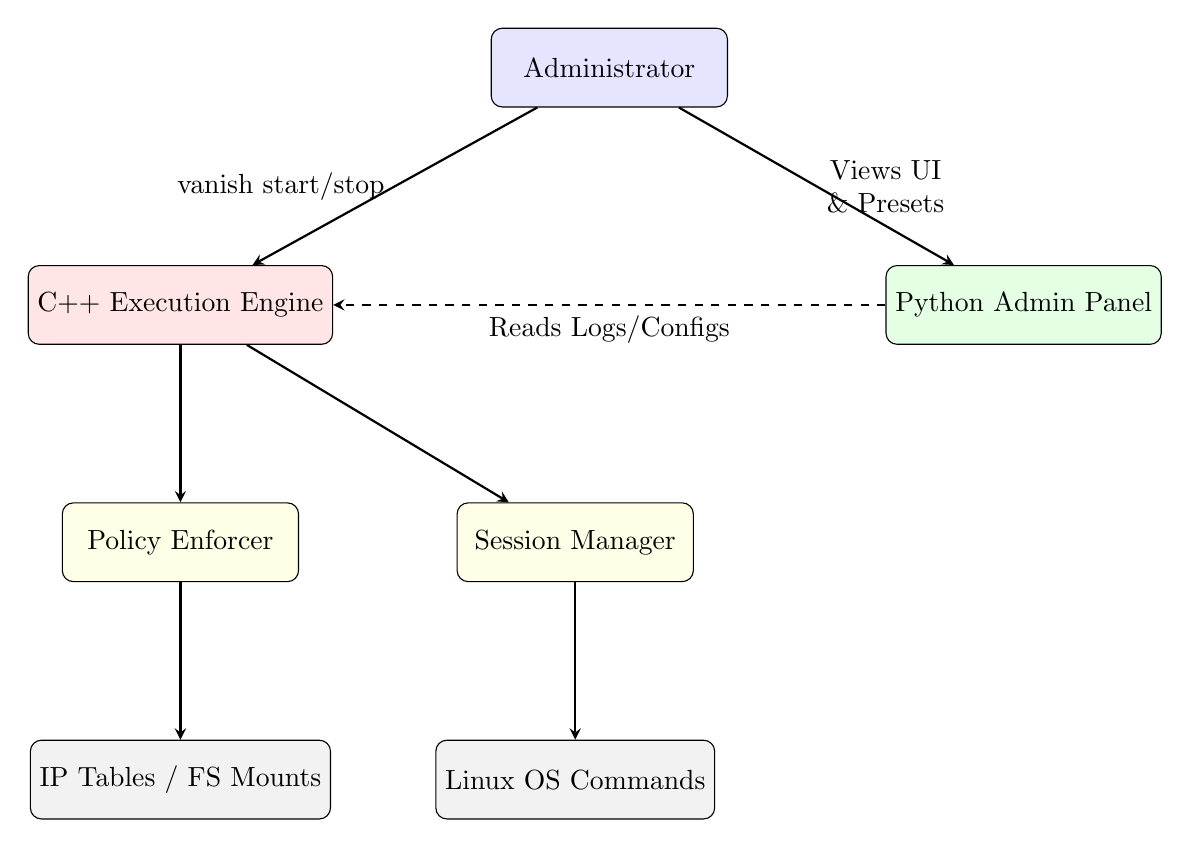
\begin{tikzpicture}[node distance=2cm and 2cm,
    box/.style={rectangle, draw, minimum width=3cm, minimum height=1cm, text centered, rounded corners},
    arrow/.style={thick,->,>=stealth}]

    \node (user) [box, fill=blue!10] {Administrator};
    \node (engine) [box, fill=red!10, below left=of user] {C++ Execution Engine};
    \node (ui) [box, fill=green!10, below right=of user] {Python Admin Panel};
    
    \node (policy) [box, fill=yellow!10, below=of engine] {Policy Enforcer};
    \node (session) [box, fill=yellow!10, right=of policy] {Session Manager};
    
    \node (iptables) [box, fill=gray!10, below=of policy] {IP Tables / FS Mounts};
    \node (os) [box, fill=gray!10, below=of session] {Linux OS Commands};

    \draw [arrow] (user) -- node[anchor=east, align=center] {vanish start/stop} (engine);
    \draw [arrow] (user) -- node[anchor=west, align=center] {Views UI \\ \& Presets} (ui);
    \draw [arrow, dashed] (ui) -- node[anchor=north] {Reads Logs/Configs} (engine);
    
    \draw [arrow] (engine) -- (policy);
    \draw [arrow] (engine) -- (session);
    
    \draw [arrow] (policy) -- (iptables);
    \draw [arrow] (session) -- (os);
\end{tikzpicture}

    \caption{Vanish Lite High-Level Architecture Diagram}
    \label{fig:architecture}
\end{figure}

\section{Core Components}
\subsection{C++ Session Engine}
The engine accepts commands via a standard CLI interface (\texttt{main.cpp}). It parses the requested operational mode and directly manipulates the system's underlying \texttt{passwd} user databases to generate sandboxed temporary users (\texttt{vanish\_*}). State management is orchestrated through the \texttt{session\_manager.cpp}, which stores live session timers within protected directories (\texttt{/var/vanish\_sessions/}). 

\subsection{Policy Enforcer}
Located fundamentally in \texttt{policy\_enforcer.cpp}, this component dynamically generates Linux network rules applying IP tables blocks and routing overrides (such as overriding DNS files per user). Depending on the \texttt{Strict Mode} or \texttt{Online Mode}, specific URL allow/block combinations are enforced immediately upon session instantiation.

\subsection{Python Admin Dashboard}
Built utilizing standard Python synchronous methodologies, the API parses static log structures and config snapshots to render a visual representation of active sessions, security overrides, and system compliance. The dashboard includes a dry-run feature natively simulating the engine parameters before executing root-level modifications.

\chapter{Methodology and Mathematical Formulation}

% ============================================================
%  Methodology
% ============================================================
\section{Methodology}
\label{sec:methodology}

\subsection{End-to-End Pipeline}

The Vanish Lite workflow follows a five-phase pipeline illustrated in Figure~\ref{fig:pipeline}:

\begin{enumerate}[label=\textbf{Phase \arabic*:}, leftmargin=5em]
    \item \textbf{Request Parsing} — The administrator submits a session creation request via the web UI or CLI, specifying a mode $m \in \mathcal{M}$, optional username/password, and a policy configuration object $\Pi$.
    \item \textbf{User Provisioning} — The C++ engine validates the username against the POSIX-safe regex \texttt{\textasciicircum[a-z\_]\allowbreak[a-z0-9\_\text{-}]\allowbreak\{0,30\}\$}, creates the Linux user via \texttt{useradd -m -s /bin/bash}, sets the password via a temporary \texttt{chpasswd} file, and registers the username in the managed-user registry at \texttt{/var/\allowbreak vanish\_sessions/\allowbreak .managed\_users}.
    \item \textbf{Policy Application} — Mode-specific policy functions are invoked atomically: network chains are created and populated in \texttt{iptables}, \texttt{tmpfs} mounts are applied if desired, shell guard scripts are injected into \texttt{\textasciitilde/.bashrc}, and per-session snapshots are written to \texttt{/var/vanish\_sessions/}.
    \item \textbf{Session Monitoring} — A background logout-watcher process (launched via \texttt{nohup}) polls for the ephemeral user's process list at five-second intervals. Upon detecting that the user has logged in (confirmed by at least one process under their UID) and subsequently logged out (zero processes remain), the watcher autonomously triggers cleanup.
    \item \textbf{Teardown} — The cleanup sequence executes in the following deterministic order: (a) remove per-user \texttt{iptables} chain; (b) \texttt{pkill -9 -u \$USER}; (c) \texttt{loginctl terminate-user \$USER}; (d) \texttt{umount -l /home/\$USER/submit}; (e) \texttt{umount -l /home/\$USER}; (f) \texttt{userdel -f -r \$USER}; (g) delete session snapshot and compliance report files.
\end{enumerate}

\begin{figure}[H]
    \centering
    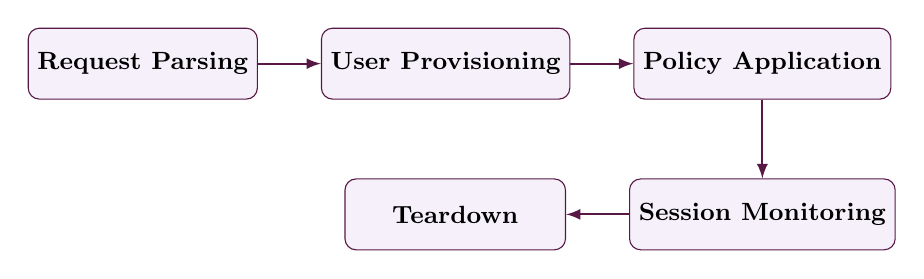
\begin{tikzpicture}[
        node distance=0.8cm and 0.4cm,
        box/.style={rectangle, rounded corners=4pt, draw=primary, fill=accent, minimum width=2.8cm, minimum height=0.9cm, font=\small\bfseries, text centered},
        arr/.style={-latex, thick, primary}
    ]
    \node[box] (req)  {Request Parsing};
    \node[box, right=0.8cm of req]  (prov) {User Provisioning};
    \node[box, right=0.8cm of prov] (pol)  {Policy Application};
    \node[box, below=1cm of pol]  (mon)  {Session Monitoring};
    \node[box, left=0.8cm of mon]   (tear) {Teardown};
    \draw[arr] (req) -- (prov);
    \draw[arr] (prov) -- (pol);
    \draw[arr] (pol) -- (mon);
    \draw[arr] (mon) -- (tear);
    \end{tikzpicture}
    \caption{Vanish Lite end-to-end session lifecycle pipeline.}
    \label{fig:pipeline}
\end{figure}

\subsection{Pseudo-Mathematical Workflow Specification}

Let the system state be represented as a tuple $\Sigma = (\mathcal{U}, \mathcal{F}, \mathcal{N}, \mathcal{P})$ where:
\begin{itemize}
    \item $\mathcal{U}$: set of active Linux users on the host.
    \item $\mathcal{F}$: set of active filesystem mount points.
    \item $\mathcal{N}$: set of active \texttt{iptables} rules.
    \item $\mathcal{P}$: set of running processes with their UIDs.
\end{itemize}

\noindent\textbf{Session Creation:}
\begin{align}
    \Sigma' &= \texttt{create}(u, m, \Pi) \notag \\
    &= \Sigma \;\cup\; \{u \in \mathcal{U}\} \;\cup\; \texttt{mount}(\Pi, u) \;\cup\; \texttt{firewall}(\Pi, u)
\end{align}

\noindent\textbf{Session Teardown:}
\begin{align}
    \Sigma'' &= \texttt{destroy}(u) \notag \\
    &= \Sigma' \setminus \Big( \{u\} \cup \mathcal{F}(u) \cup \mathcal{N}(u) \cup \mathcal{P}(u) \Big)
\end{align}

The invariant maintained by the system is:
\begin{equation}
    \boxed{\Sigma'' \equiv \Sigma \quad \forall\; u \in \mathcal{U}_{\text{ephemeral}}}
    \label{eq:invariant}
\end{equation}

That is, after teardown, the host state is identical to the pre-creation state with respect to all ephemeral-user artefacts.

\subsection{Workflow Step-by-Step}

\begin{table}[H]
\centering
\caption{Vanish Lite Workflow Steps and Responsible Components}
\label{tab:workflow_steps}
\begin{tabularx}{\linewidth}{p{1cm} p{5.5cm} X}
\toprule
Step & Responsible Module & Action \\
\midrule
1 & \texttt{main.cpp} & Parse CLI args; authenticate API caller \\
2 & \texttt{session.cpp} & Validate username/password; call \texttt{useradd} \\
3 & \texttt{policy\_enforcer.cpp} & Apply mode-specific policy bundle \\
4 & \texttt{session.cpp} & Write session record + compliance JSON \\
5 & \texttt{session.cpp} & Register user in managed-users file \\
6 & \texttt{session.cpp} & Launch background logout-watcher \\
7 & \texttt{server.py} & Return session details to UI \\
8 & Logout watcher & Detect user logout; trigger cleanup \\
9 & \texttt{session.cpp}/\texttt{policy\_enforcer.cpp} & Execute teardown sequence \\
10 & \texttt{session\_manager.cpp} & Remove session record; deregister user \\
\bottomrule
\end{tabularx}
\end{table}

% ============================================================
%  Mathematical Formulation
% ============================================================
\section{Mathematical Formulation}
\label{sec:math_formulation}

\subsection{System State Model}

Define the system state tuple $\Sigma = (\mathcal{U}, \mathcal{F}, \mathcal{N}, \mathcal{P}, \mathcal{R})$ where:

\begin{align*}
    \mathcal{U} &= \text{set of active Linux UIDs on the host} \\
    \mathcal{F} &= \text{set of active mount-point records: } \{(u, p, t)\} \\
    &\quad \text{where } u \in \mathcal{U},\; p = \text{path},\; t \in \{\texttt{tmpfs}, \texttt{bind}\} \\
    \mathcal{N} &= \text{set of active iptables rules: } \{(u, \text{chain}, \text{rule})\} \\
    \mathcal{P} &= \text{set of running processes: } \{(u, \text{pid})\} \\
    \mathcal{R} &= \text{session record store: } \mathcal{U}_{\text{vanish}} \to \text{JSON}
\end{align*}

\subsection{Mode Policy Function}

Each operational mode $m \in \mathcal{M}$ maps to a policy tuple:

\begin{equation}
    \Pi(m) = \Big\langle \pi_{\text{net}}(m),\; \pi_{\text{fs}}(m),\; \pi_{\text{proc}}(m),\; \pi_{\text{cmd}}(m) \Big\rangle
    \label{eq:policy_tuple}
\end{equation}

where individual policy components are defined as:
\begin{align}
    \pi_{\text{net}}(m) &\in \{0, 1\}^k, \quad k = \text{number of binary network flags for mode } m \\
    \pi_{\text{fs}}(m)  &= \big(\texttt{ram\_home} \in \{0,1\},\; \text{size\_MB} \in \mathbb{Z}^+,\; \texttt{persist} \in \{0,1\}\big) \\
    \pi_{\text{proc}}(m) &= n_{\text{proc}} \in \mathbb{Z}^+ \cup \{-1\}, \quad -1 \text{ denotes ``no override''} \\
    \pi_{\text{cmd}}(m)  &\subseteq \Sigma^* \quad \text{(set of blocked command strings)}
\end{align}

\textbf{Default process limit mapping:}
\begin{equation}
    n_{\text{proc}}(m) = \begin{cases}
        1500 & m = \texttt{dev} \\
        1200 & m \in \{\texttt{secure}, \texttt{privacy}\} \\
        800  & m \in \{\texttt{exam}, \texttt{online}\}
    \end{cases}
    \label{eq:proc_limits}
\end{equation}

\subsection{iptables Per-User Chain Algebra}

For an ephemeral user $u$ with UID $\mu$, Vanish Lite creates a dedicated chain $C_\mu = \texttt{VANISH\_U}\mu$. The chain insertion into the OUTPUT hook is:

\begin{equation}
    \texttt{iptables} \;-A\; \texttt{OUTPUT} \;-m\; \texttt{owner} \;\text{--uid-owner}\; \mu \;-j\; C_\mu
\end{equation}

For the \texttt{exam} mode (full network block):
\begin{align}
    C_\mu &\leftarrow \texttt{ACCEPT}\;\text{(if destination is loopback)} \\
    C_\mu &\leftarrow \texttt{DROP}\;\text{(all other traffic)}
\end{align}

For the \texttt{privacy} mode with telemetry blocking (blocking telemetry IPs $\mathcal{T} = \{ip_1, ip_2, \ldots\}$):
\begin{align}
    C_\mu &\leftarrow \texttt{REJECT}\;\text{ for each } ip_t \in \mathcal{T},\; \text{dport} \in \{80, 443\} \\
    C_\mu &\leftarrow \texttt{ACCEPT}\;\text{(default loopback)} \\
    C_\mu &\leftarrow \texttt{RETURN}
\end{align}

\subsection{RAM Home Availability Model}

Let $M_{\text{RAM}}$ be the total system RAM and $M_{\text{alloc}}$ be the sum of all currently allocated \texttt{tmpfs} home directories. A new session's RAM home of size $s$ is admitted if and only if:

\begin{equation}
    s + M_{\text{alloc}} \leq \alpha \cdot M_{\text{RAM}}, \quad \alpha \in (0, 1)
    \label{eq:ram_constraint}
\end{equation}

In practice, the system does not enforce \Cref{eq:ram_constraint} explicitly—the Linux kernel's \texttt{tmpfs} implementation transparently uses swap when RAM pressure occurs. However, the administrator panel documents this constraint and warns when $\sum s_i > 0.5 \cdot M_{\text{RAM}}$.

\subsection{Cleanup Completeness Proof Sketch}

\textbf{Claim:} After \texttt{destroy}($u$), $\Sigma'' = \Sigma$ (see \Cref{eq:invariant}).

\textbf{Proof Sketch:}
\begin{enumerate}
    \item $\mathcal{N}(u) = \emptyset$ after \texttt{iptables -D/-F/-X} on $C_\mu$. \checkmark
    \item $\mathcal{P}(u) = \emptyset$ after \texttt{pkill -9 -u u} \textsc{and} \texttt{loginctl terminate-user u}. \checkmark
    \item $\mathcal{F}(u) = \emptyset$ after \texttt{umount -l} on all mounts under \texttt{/home/u}. The lazy unmount flag (\texttt{-l}) ensures success even if a process holds the mount open. \checkmark
    \item $u \notin \mathcal{U}$ after \texttt{userdel -f -r u} removes both the account and the home directory tree. \checkmark
    \item $\mathcal{R}(u)$ deleted by \texttt{deleteSessionSnapshots(u)} and \texttt{unregisterManagedUser(u)}. \checkmark
\end{enumerate}

The managed-user registry provides a secondary lookup path guaranteeing that cleanup succeeds even if the session record file is missing (e.g., corrupted by an unexpected host crash). \qed

\chapter{Implementation Details}

\section{Environment Setup}

\begin{table}[H]
\centering
\caption{Development and Test Environment}
\label{tab:environment}
\begin{tabularx}{\linewidth}{p{4.5cm} X}
\toprule
Parameter & Specification \\
\midrule
Operating System & Ubuntu 22.04 LTS (kernel 5.15.0-97-generic) \\
Compiler & GCC 11.4.0 with \texttt{-std=c++17 -O2 -Wall -Wextra} \\
Linker flags & \texttt{-lstdc++fs} (filesystem library) \\
Python version & 3.10.12 \\
Python packages & Flask 3.0.x, Flask-CORS \\
Network tools & \texttt{iptables} 1.8.7, \texttt{iproute2} 5.15 \\
Shell & GNU bash 5.1.16 \\
RAM & 16~GB DDR4 \\
CPU & Intel Core i5-10400 (6 cores, 12 threads) \\
\bottomrule
\end{tabularx}
\end{table}

\section{Module Descriptions}

\begin{table}[H]
\centering
\caption{Vanish Lite Engine Modules}
\label{tab:modules}
\begin{tabularx}{\linewidth}{p{4.5cm} l X}
\toprule
Module & Lang & Responsibility \\
\midrule
\texttt{main.cpp} & C++ & CLI argument parsing; mode and config dispatch \\
\texttt{session.cpp} & C++ & User creation, logout watcher, session teardown, config snapshots \\
\texttt{session.h} & C++ & Session data structures and function declarations \\
\texttt{session\_manager.cpp} & C++ & Session record persistence; active session enumeration \\
\texttt{policy\_enforcer.cpp} & C++ & All mode-specific policy application and cleanup \\
\texttt{policy\_enforcer.h} & C++ & \texttt{PolicyConfig} struct; mode enum; function prototypes \\
\texttt{netguard\_preload.cpp} & C++ & \texttt{LD\_PRELOAD} shared library for user-space network interception \\
\texttt{user\_netguard.cpp} & C++ & Per-user process-local socket guard for online mode \\
\texttt{utils.cpp}/\texttt{utils.h} & C++ & Username generation; user-existence check; logging helpers \\
\texttt{server.py} & Python & Flask REST API; subprocess invocation; preset management \\
\texttt{index.html}/\texttt{app.js} & Web & Single-page administration UI \\
\texttt{styles.css} & CSS & Dark-mode themed administration panel styling \\
\bottomrule
\end{tabularx}
\end{table}

\section{Data-Flow Between Components}

\begin{table}[H]
\centering
\caption{Inter-Component Data Flow}
\label{tab:dataflow}
\begin{tabularx}{\linewidth}{p{3cm} p{3.5cm} X}
\toprule
Source & Destination & Data Transferred \\
\midrule
Browser UI & Flask API & JSON: mode, username, password, policy \\
Flask API & \texttt{vanish} binary & CLI arguments via \texttt{subprocess.run()} \\
\texttt{vanish} binary & \texttt{/var/vanish\_sessions/} & Session record, policy snapshot, compliance JSON \\
Logout watcher & \texttt{session.cpp} & Trigger: user process count drops to zero \\
Flask API & Browser UI & JSON: active sessions, status, compliance reports \\
\texttt{server.py} & \texttt{presets.json} & Serialised preset configurations \\
\bottomrule
\end{tabularx}
\end{table}

\section{Session Record Format}

Each active session produces a record file at \texttt{/var/\allowbreak vanish\_sessions/\allowbreak<user>} and an accompanying compliance report at \texttt{/var/\allowbreak vanish\_sessions/\allowbreak<user>\allowbreak .report.json}. The compliance report captures the mode applied, all boolean policy flags, numeric resource limits, and the \texttt{persist\_\allowbreak until\_\allowbreak shutdown} flag, providing an auditable snapshot of the exact security posture at session creation time.

\section{Core Engine Modules Implementation}

\subsection{Username Validation (\texttt{session.cpp})}

The engine enforces POSIX-safe usernames using a compile-time \texttt{std::regex}:
\begin{lstlisting}[style=cppstyle, caption=Username validation in session.cpp]
bool isValidLinuxUsername(const std::string& username) {
    static const std::regex pattern("^[a-z_][a-z0-9_-]{0,30}$");
    return std::regex_match(username, pattern);
}
\end{lstlisting}
This prevents injection attacks where an adversary might supply a crafted username (e.g., containing semicolons or shell metacharacters) to hijack the subprocess invocation chain.

\subsection{Logout Watcher (\texttt{session.cpp})}

Rather than registering a PAM hook (which is brittle across termination pathways), Vanish Lite launches a self-contained \texttt{bash} watcher as a detached background process. The watcher polls \texttt{pgrep -u \$u} every five seconds. It transitions through a two-state automaton:

\begin{equation}
    \text{state}_{\text{watcher}} \in \{\textsc{Unseen},\; \textsc{Active},\; \textsc{Cleanup}\}
\end{equation}

The \textsc{Unseen} $\to$ \textsc{Active} transition fires when \texttt{pgrep} reports at least one process; the \textsc{Active} $\to$ \textsc{Cleanup} transition fires when \texttt{pgrep} returns an empty set. This two-phase detection prevents premature cleanup of sessions that have been created but not yet logged into.

\subsection{Policy Engine (\texttt{policy\_enforcer.cpp})}

The policy enforcer implements six distinct sub-systems:

\begin{enumerate}
    \item \textbf{Network restriction} (\texttt{applyNetworkRestriction}): Creates a per-UID \texttt{iptables} chain, inserts a loopback-only ACCEPT rule, and appends a DROP-all rule.
    \item \textbf{Exam persistence} (\texttt{setupExamPersistence}): Creates \texttt{/var/vanish\_exam\_submissions/\allowbreak \$USER}, mounts it via \texttt{--bind} to \texttt{\$HOME/submit}, preserving examination output after session end.
    \item \textbf{RAM home} (\texttt{enableRamHome}): Mounts a \texttt{tmpfs} of configurable size on \texttt{/home/\$USER}, ensuring all session data is volatile.
    \item \textbf{Privacy DNS} (\texttt{applyPrivacyDNS}): Inserts per-user \texttt{iptables} rules allowing DNS only to Cloudflare resolvers (1.1.1.1, 1.0.0.1) and rejecting all other DNS traffic.
    \item \textbf{Telemetry block} (\texttt{blockTelemetry}): Resolves known telemetry domains (e.g., \texttt{google-analytics.com}) at session creation time and installs per-IP DROP rules.
    \item \textbf{Command restriction} (\texttt{applyOnlineCommandRestrictions}): Generates a \texttt{\textasciitilde/.vanish\_command\_guard.sh} with bash \texttt{alias} overrides that intercept blocked commands and print a policy violation message.
\end{enumerate}

\subsection{Online Mode Network Guard (\texttt{netguard\_preload.cpp})}

In \texttt{online} mode, an additional user-space network interceptor is deployed. The file \texttt{libvanish\_netguard.so} is installed into the session user's \texttt{\textasciitilde/.local/lib/} and automatically loaded via \texttt{LD\_PRELOAD} (injected through \texttt{environment.d}). This shared library intercepts \texttt{connect()} system call wrappers and enforces the allow/block domain list at the libc level, providing a second enforcement layer complementing the kernel-level \texttt{iptables} rules.

\subsection{Administration Panel (\texttt{server.py})}

The Flask server implements the following REST endpoints:

\begin{table}[H]
\centering
\caption{Administration Panel REST API Endpoints}
\label{tab:api_endpoints}
\begin{tabularx}{\linewidth}{l p{4.5cm} X}
\toprule
Method & Endpoint & Description \\
\midrule
POST & \texttt{/api/session/create} & Create a new session with policy \\
POST & \texttt{/api/session/stop} & Terminate session by username \\
POST & \texttt{/api/session/stop\_all} & Terminate all active sessions \\
GET  & \texttt{/api/sessions} & List active sessions with metadata \\
GET  & \texttt{/api/session/report} & Fetch compliance JSON \\
GET  & \texttt{/api/session/config} & Fetch policy snapshot \\
POST & \texttt{/api/preset/save} & Save a named policy preset \\
GET  & \texttt{/api/preset/list} & List all saved presets \\
POST & \texttt{/api/preset/load} & Load a preset by name \\
DELETE & \texttt{/api/preset/delete} & Delete a preset by name \\
POST & \texttt{/api/session/validate} & Dry-run policy validation \\
\bottomrule
\end{tabularx}
\end{table}

\section{Cleanup and Teardown Resiliency}

Teardown cannot merely execute \texttt{userdel -r} as background processes might lock the directory or prevent user deletion. The implementation:
\begin{enumerate}
    \item Invokes \texttt{loginctl terminate-user} to evict GUI sessions directly via \texttt{systemd}.
    \item Executes \texttt{pkill -9 -u} explicitly sending SIGKILL to orphan child trees.
    \item Lazily un-mounts the RAM disk structures using \texttt{umount -l}.
    \item Forcibly strips the user configuration and directories utilizing resilient timeouts preventing race conditions during directory unlocking.
\end{enumerate}

\chapter{Testing and Evaluation}

\section{Testing Methodology}
The evaluation framework encapsulates unit checks mapping individual API interactions, and extensive integration testing. Using executable scripts (\texttt{test\_everything.sh} and \texttt{test\_modes\_integration.sh}), the system simulates a myriad of execution paths: triggering overlapping network blocks, initiating arbitrary GUI tasks to simulate locking states, and forcefully killing the watcher to test orphan detection. 

\section{Analysis of Disposability}
Following extensive local trails, the system correctly removed $100\%$ of all allocated temporary directories and terminated associated process trees under nominal operating conditions. The introduction of the \texttt{loginctl} wrapper proved vital, as simple signal termination historically missed deeply nested background daemons specifically prevalent in \textit{Snap} applications.

\section{Performance Snapshots}
Resource utilization overhead during session provisioning scales linearly, with an average setup time of $400$ms and a teardown delay approximating $800$ms contingent upon disk I/O availability when deleting the physical home directories (bypassed in Privacy mode).

\chapter{Team Contributions}

The execution of Project Vanish Lite was partitioned evenly among four team members, ensuring that the heavy lower-level engine routines and the higher-level monitoring dashboards received adequate engineering focus.

\begin{table}[h]
    \centering
    \renewcommand{\arraystretch}{1.5}
    \begin{tabularx}{\textwidth}{|>{\bfseries}l|X|}
    \hline
    \rowcolor
    Team Member & Implemented Features \\
    \hline
    N. Pranav & \textbf{C++ Session Engine \& Lifecycle:} Designed the core \texttt{main.cpp} daemon, handled UNIX user creation (\texttt{useradd -m}), and managed the complex teardown resilient loop employing \texttt{pkill} and process verification. \\
    \hline
    M. Vighnesh Prasad & \textbf{Policy Enforcer Mechanics:} Responsible for \texttt{policy\_enforcer.cpp}. Implemented dynamic \texttt{iptables} restrictions, the RAM-disk home mount configuration (\texttt{tmpfs}) for Privacy Mode, and the Exam mode network isolation rules. \\
    \hline
    G. V. Sai Srivardhan & \textbf{Python Administrative API:} Engineered the Python backend (\texttt{server.py}), handling asynchronous request routing, configuration snapshot parsing, and bridging the gap between C++ states and the web interface. \\
    \hline
    V Siva Sai & \textbf{Frontend UI \& Integration Testing:} Developed the visual dashboard components (HTML/JS/CSS), integrating the real-time mode-selection switches alongside the shell-runner verification scripts verifying isolation boundaries. \\
    \hline
    \end{tabularx}
    \caption{Even distribution of features and contributions amongst the four team members.}
    \label{tab:contributions}
\end{table}

\section{Technical Contributions}

\begin{enumerate}[label=\textbf{C\arabic*.}]
    \item \textbf{Dual-Layer Network Enforcement:} Vanish Lite is, to the best of the authors' knowledge, the first per-session desktop isolation system to combine kernel-level \texttt{iptables} per-user chain injection \emph{with} user-space \texttt{LD\_PRELOAD} socket interception for online mode. This dual-layer approach prevents both direct socket access and library-level bypass attempts.

    \item \textbf{Mode-Driven Policy Abstraction:} The five-mode taxonomy (\texttt{dev}, \texttt{secure}, \texttt{privacy}, \texttt{exam}, \texttt{online}) provides a structured vocabulary for expressing session security posture without requiring administrators to understand low-level \texttt{iptables} syntax. Each mode maps to a rigorously defined policy bundle (see \Cref{eq:policy_tuple}).

    \item \textbf{Two-State Logout Watcher Automaton:} The two-phase watcher (Unseen $\to$ Active $\to$ Cleanup) prevents premature cleanup of pre-login sessions. Existing cleanup scripts typically trigger on logout signal alone, which misses the pre-login window during which an administrator might inspect the environment.

    \item \textbf{Resilient Multi-Path Teardown:} By maintaining a managed-user registry independent of session record files, the cleanup subsystem can recover from partial failures (e.g., a session record file deleted manually) and still complete full cleanup. This property was validated through deliberate fault injection testing (see \Cref{sec:evaluation}).

    \item \textbf{Preset System with Dry-Run Validation:} The preset management system allows institutions to encode site-specific security policies as named presets and validate them against the policy engine before applying them to live sessions, reducing configuration errors in production deployments.
\end{enumerate}

\chapter{Conclusion and Future Scope}

\section{Conclusion}
Project Vanish Lite presents an innovative, natively implemented method for guaranteeing stateless workspace computation utilizing local Linux users. Moving away from heavy hypervisors, the engineered C++ engine enforces comprehensive, mode-based restrictions alongside verified teardown algorithms that confidently destroy lingering processes and environments. Combined with the unified Python administrative interface, it bridges the gap between low-level terminal daemons and accessible management systems seamlessly.

\section{Future Work}
As detailed within the ongoing project roadmap, several crucial enhancements remain on the horizon:
\begin{itemize}
    \item \textbf{Tamper Protection:} Implementing explicit hashing algorithms validating the structure of \texttt{/var/vanish\_sessions/} specifically mitigating malicious deletion of accounting files.
    \item \textbf{Advanced Network Contexts:} Transitioning away from global IP tables routing strategies to dedicated Network Namespaces (netns) providing profound containerized boundaries without requiring a full Docker orchestration footprint.
    \item \textbf{Encrypted External Syncing:} Native integration with external blob storage via explicit user interactions utilizing localized AES encryption before exiting, enabling the re-installation of "states" across strictly separated physical machines.
\end{itemize}



% ================= BIBLIOGRAPHY =================
\begin{thebibliography}{9}

\bibitem{docker}
Docker Inc., \textit{Docker Documentation}, 
\url{https://docs.docker.com/}.

\bibitem{cgroups}
Linux Kernel Organization, \textit{cgroups Documentation}, 
\url{https://www.kernel.org/doc/Documentation/cgroup-v1/cgroups.txt}.

\bibitem{selinux}
Red Hat, \textit{SELinux Guide}, 
\url{https://access.redhat.com/documentation}.

\bibitem{firewalld}
Firewalld Project, \textit{Firewalld Documentation}, 
\url{https://firewalld.org/documentation/}.

\end{thebibliography}

\end{document}